\vspace{-1.1em}
\section{Biographie du D\'eveloppeur}\label{chap:biography}
\vspace{-0.9em}
\begin{figure}[!htpb]
\centering
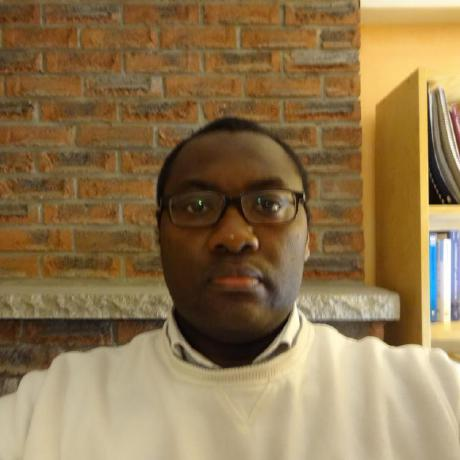
\includegraphics[scale=0.35]{../images/XavierNOUNDOU-2}
\caption{Portrait de Xavier}~\label{fig:xaviernoumbis}
\end{figure}

\company{NOUMBISSI NOUNDOU Xavier} est Camerounais.
Il est n\'e en $1983$, et est d\'etenteur d'un
dipl\^ome d'ing\'enieur de conception en informatique
(\emph{\diplominformatiker} [\diplinf]) de \company{l'universit\'e de Br\^eme}
(Bremen, Allemagne).

Pendant ses \'etudes de \diplinf,
Xavier a travaill\'e pendant $25$~mois comme
d\'eveloppeur--logiciel (temps--partiel) \`a
\company{\bergmann} dans la ville de Rellingen
(Hambourg, Allemagne).

Apr\`es l'obtention de son \diplinf, Xavier a travaill\'e
$21$~mois comme d\'eveloppeur--logiciel--junior \`a
\company{\siemens} dans la ville d'Erlangen (Bavi\`ere, Allemagne).

Xavier a quitt\'e ''\siemens'' en $2009$ pour poursuivre
des \'etudes doctorales en analyse statique des programmes
informatiques au laboratoire de recherche \company{Watform}
de \company{l'universit\'e de Waterloo}.

En $2012$, Xavier a travaill\'e $8$ mois en tant
que stagiaire doctorant dans l'\'equipe de compilation 
\emph{Java Just--In--Time Compiler (J~$9$)} de
\company{IBM Toronto Lab} \`a Markham (Ontario, Canada).

Xavier quitte le labratoire de recherche ''Watform''
en Mars~$2015$, pour fonder l'entreprise d'\'edition
de syst\`emes--logiciels \textbf{\yerenlabs}.

Xavier lit, \'ecrit, et parle courament l'Allemand,
l'Anglais, et le Fran\c{c}ais.
